
\section{Architecture Integration}

\subsection{Model Support}

\begin{table}[H]
\centering
\small
\begin{tabular}{llllllll}
\toprule
\textbf{Model} & \textbf{Layers} & \textbf{$d$} & \textbf{$H$} & \textbf{$H_{kv}$} & \textbf{Nested?} & \textbf{Conv1D?} & \textbf{RoPE?} \\
\midrule
DistilBERT-base & 6 & 768 & 12 & 12 & No & No & No \\
RoBERTa-base & 12 & 768 & 12 & 12 & Yes & No & No \\
GPT-2 & 12 & 768 & 12 & 12 & No & Yes & No \\
Qwen3.5-0.8B & 24 & 1024 & 8 & 2 & No & No & Yes \\
\bottomrule
\end{tabular}
\end{table}

\subsection{DistilBERT (Flat)}

\begin{lstlisting}
distilbert.transformer.layer.0.attention
+-- q\_lin  (Linear 768 $\to$ 768)
+-- k\_lin  (Linear 768 $\to$ 768)
+-- v\_lin  (Linear 768 $\to$ 768)
+-- out\_lin (Linear 768 $\to$ 768)
\end{lstlisting}

\textbf{Extraction:}
\begin{lstlisting}
w\_q = src.q\_lin.weight.data
w\_k = src.k\_lin.weight.data
w\_v = src.v\_lin.weight.data
w\_o = src.out\_lin.weight.data
\end{lstlisting}

\texttt{is\_nested\_encoder = False}.

\subsection{RoBERTa (Nested)}

\begin{lstlisting}
roberta.encoder.layer.0.attention
+-- self
|   +-- query
|   +-- key
|   +-- value
+-- output
    +-- dense
\end{lstlisting}

\textbf{Extraction:}
\begin{lstlisting}
src\_inner = src.self
w\_q = src\_inner.query.weight.data
w\_k = src\_inner.key.weight.data
w\_v = src\_inner.value.weight.data
w\_o = src.output.dense.weight.data
\end{lstlisting}

\textbf{Nested detection:} \texttt{hasattr(src, "self") and hasattr(src.self, "query")}.

\texttt{is\_nested\_encoder = True}. Forward returns raw context; outer 
\texttt{output.dense} applies projection.

\subsection{GPT-2 (Causal Conv1D)}

\begin{lstlisting}
transformer.h.0.attn
+-- c\_attn  (Conv1D 768 $\to$ 2304)
+-- c\_proj  (Conv1D 768 $\to$ 768)
\end{lstlisting}

\textbf{Extraction:}
\begin{lstlisting}
weight = src.c\_attn.weight.data
if weight.shape[1] == 3 * hidden\_size:   # Conv1D stores (in, out)
    weight = weight.t()
q\_w, k\_w, v\_w = weight.chunk(3, dim=0)
w\_o = src.c\_proj.weight.data
\end{lstlisting}

\texttt{is\_nested\_encoder = False}.

\subsection{Qwen3.5 (GQA + RoPE)}

\begin{lstlisting}
model.layers.0.self\_attn
+-- q\_proj  (Linear 1024 $\to$ 2048)
+-- k\_proj  (Linear 1024 $\to$ 512)
+-- v\_proj  (Linear 1024 $\to$ 512)
+-- o\_proj  (Linear 2048 $\to$ 1024)
\end{lstlisting}

\textbf{GQA dimension match:}
\begin{lstlisting}
if w\_k\_f.shape[0] \textgreater{} self.kv\_dim:
    rep = w\_k\_f.shape[0] // self.kv\_dim
    w\_k\_f = w\_k\_f.view(self.kv\_dim, rep, -1).mean(dim=1)
\end{lstlisting}

\textbf{RoPE applied after up-projection} via \texttt{position\_embeddings} in kwargs.

\texttt{is\_nested\_encoder = False}.

\subsection{Injection Hook}

\begin{lstlisting}
def inject\_mla(layer, model\_config, comp\_config=None, old\_attn=None, ...):
    rank = getattr(comp\_config, "mla\_rank", 128) if comp\_config else 128
    new\_attn = MLAAttention(model\_config, rank=rank)
    
    src\_attn = old\_attn or getattr(layer, "attention", getattr(layer, "self", None))
    if src\_attn is not None:
        new\_attn.copy\_weights(src\_attn)
        p = next(src\_attn.parameters(), None)
        if p is not None:
            new\_attn.to(device=p.device, dtype=p.dtype)
    
    if hasattr(layer, "attention"):
        if hasattr(layer.attention, "self"):
            layer.attention.self = new\_attn
        else:
            layer.attention = new\_attn
    elif hasattr(layer, "self"):
        layer.self = new\_attn
    
    return new\_attn
\end{lstlisting}

\textbf{Note.} This injection hook is \textbf{single-layer only}. Whole-model traversal 
is the caller's responsibility.

\subsection{Failure Modes}

\begin{table}[H]
\centering
\small
\begin{tabular}{lll}
\toprule
\textbf{Failure} & \textbf{Detection} & \textbf{Response} \\
\midrule
Missing Q/K/V & \texttt{copy\_weights} raises & Abort \\
Near-zero Frobenius & Norm check \textless{} 1e-4 & Raise \\
Wrong Conv1D & \texttt{hasattr(src, "c\_attn")} & Handle \\
Missing out\_proj (nested) & \texttt{is\_nested\_encoder} & Identity matrix \\
GQA dimension mismatch & Shape check & Mean-pool \\
\bottomrule
\end{tabular}
\end{table}

\subsection{Registry}

\begin{lstlisting}
@ATTENTION\_REGISTRY.register("mla")
@ATTENTION\_REGISTRY.register("mla\_attention")
class MLAAttention(BaseAttention):
    ...

@ATTENTION\_REGISTRY.register("mla\_inject")
def inject\_mla(...):
    ...
\end{lstlisting}

\subsection{LoRA Recovery Integration}

MLA integrates with the framework's LoRA recovery:

\begin{enumerate}
\item MLA initialization $\to$ frozen base, trainable LoRA on Q/O.
\item Recovery fine-tuning trains LoRA + \texttt{output\_scale}.
\item Evaluation uses the fine-tuned model.

\end{enumerate}
\subsection{Cross-Attention}

MLA does \textbf{not} support cross-attention. Encoder-decoder models (T5, BART) 
are not applicable.

\subsection{Comparison with Original DeepSeek-V2 MLA}

\begin{table}[H]
\centering
\small
\begin{tabular}{lll}
\toprule
\textbf{Aspect} & \textbf{Original} & \textbf{Our reproduction} \\
\midrule
Target architecture & DeepSeek-V2 & Four families \\
Latent dim & 512 (V2), 1536 (V3) & 32 \\
RoPE on K & Decomposed & After projection \\
GQA & Native & Supported via pool \\
Output scale & Not specified & Trainable scalar \\
\bottomrule
\end{tabular}
\end{table}

\textbf{Differences from original.}

\begin{enumerate}
\item \textbf{Latent dimension.} We use 32 instead of 512.
\item \textbf{RoPE handling.} The original applies RoPE on a decoupled head
  dimension; we apply it uniformly after up-projection.
\item \textbf{Multi-architecture support.} The original does not target DistilBERT,
  RoBERTa, or GPT-2.
\end{enumerate}
\begin{lstlisting}

---
\end{lstlisting}

\begin{figure}[H]
\centering
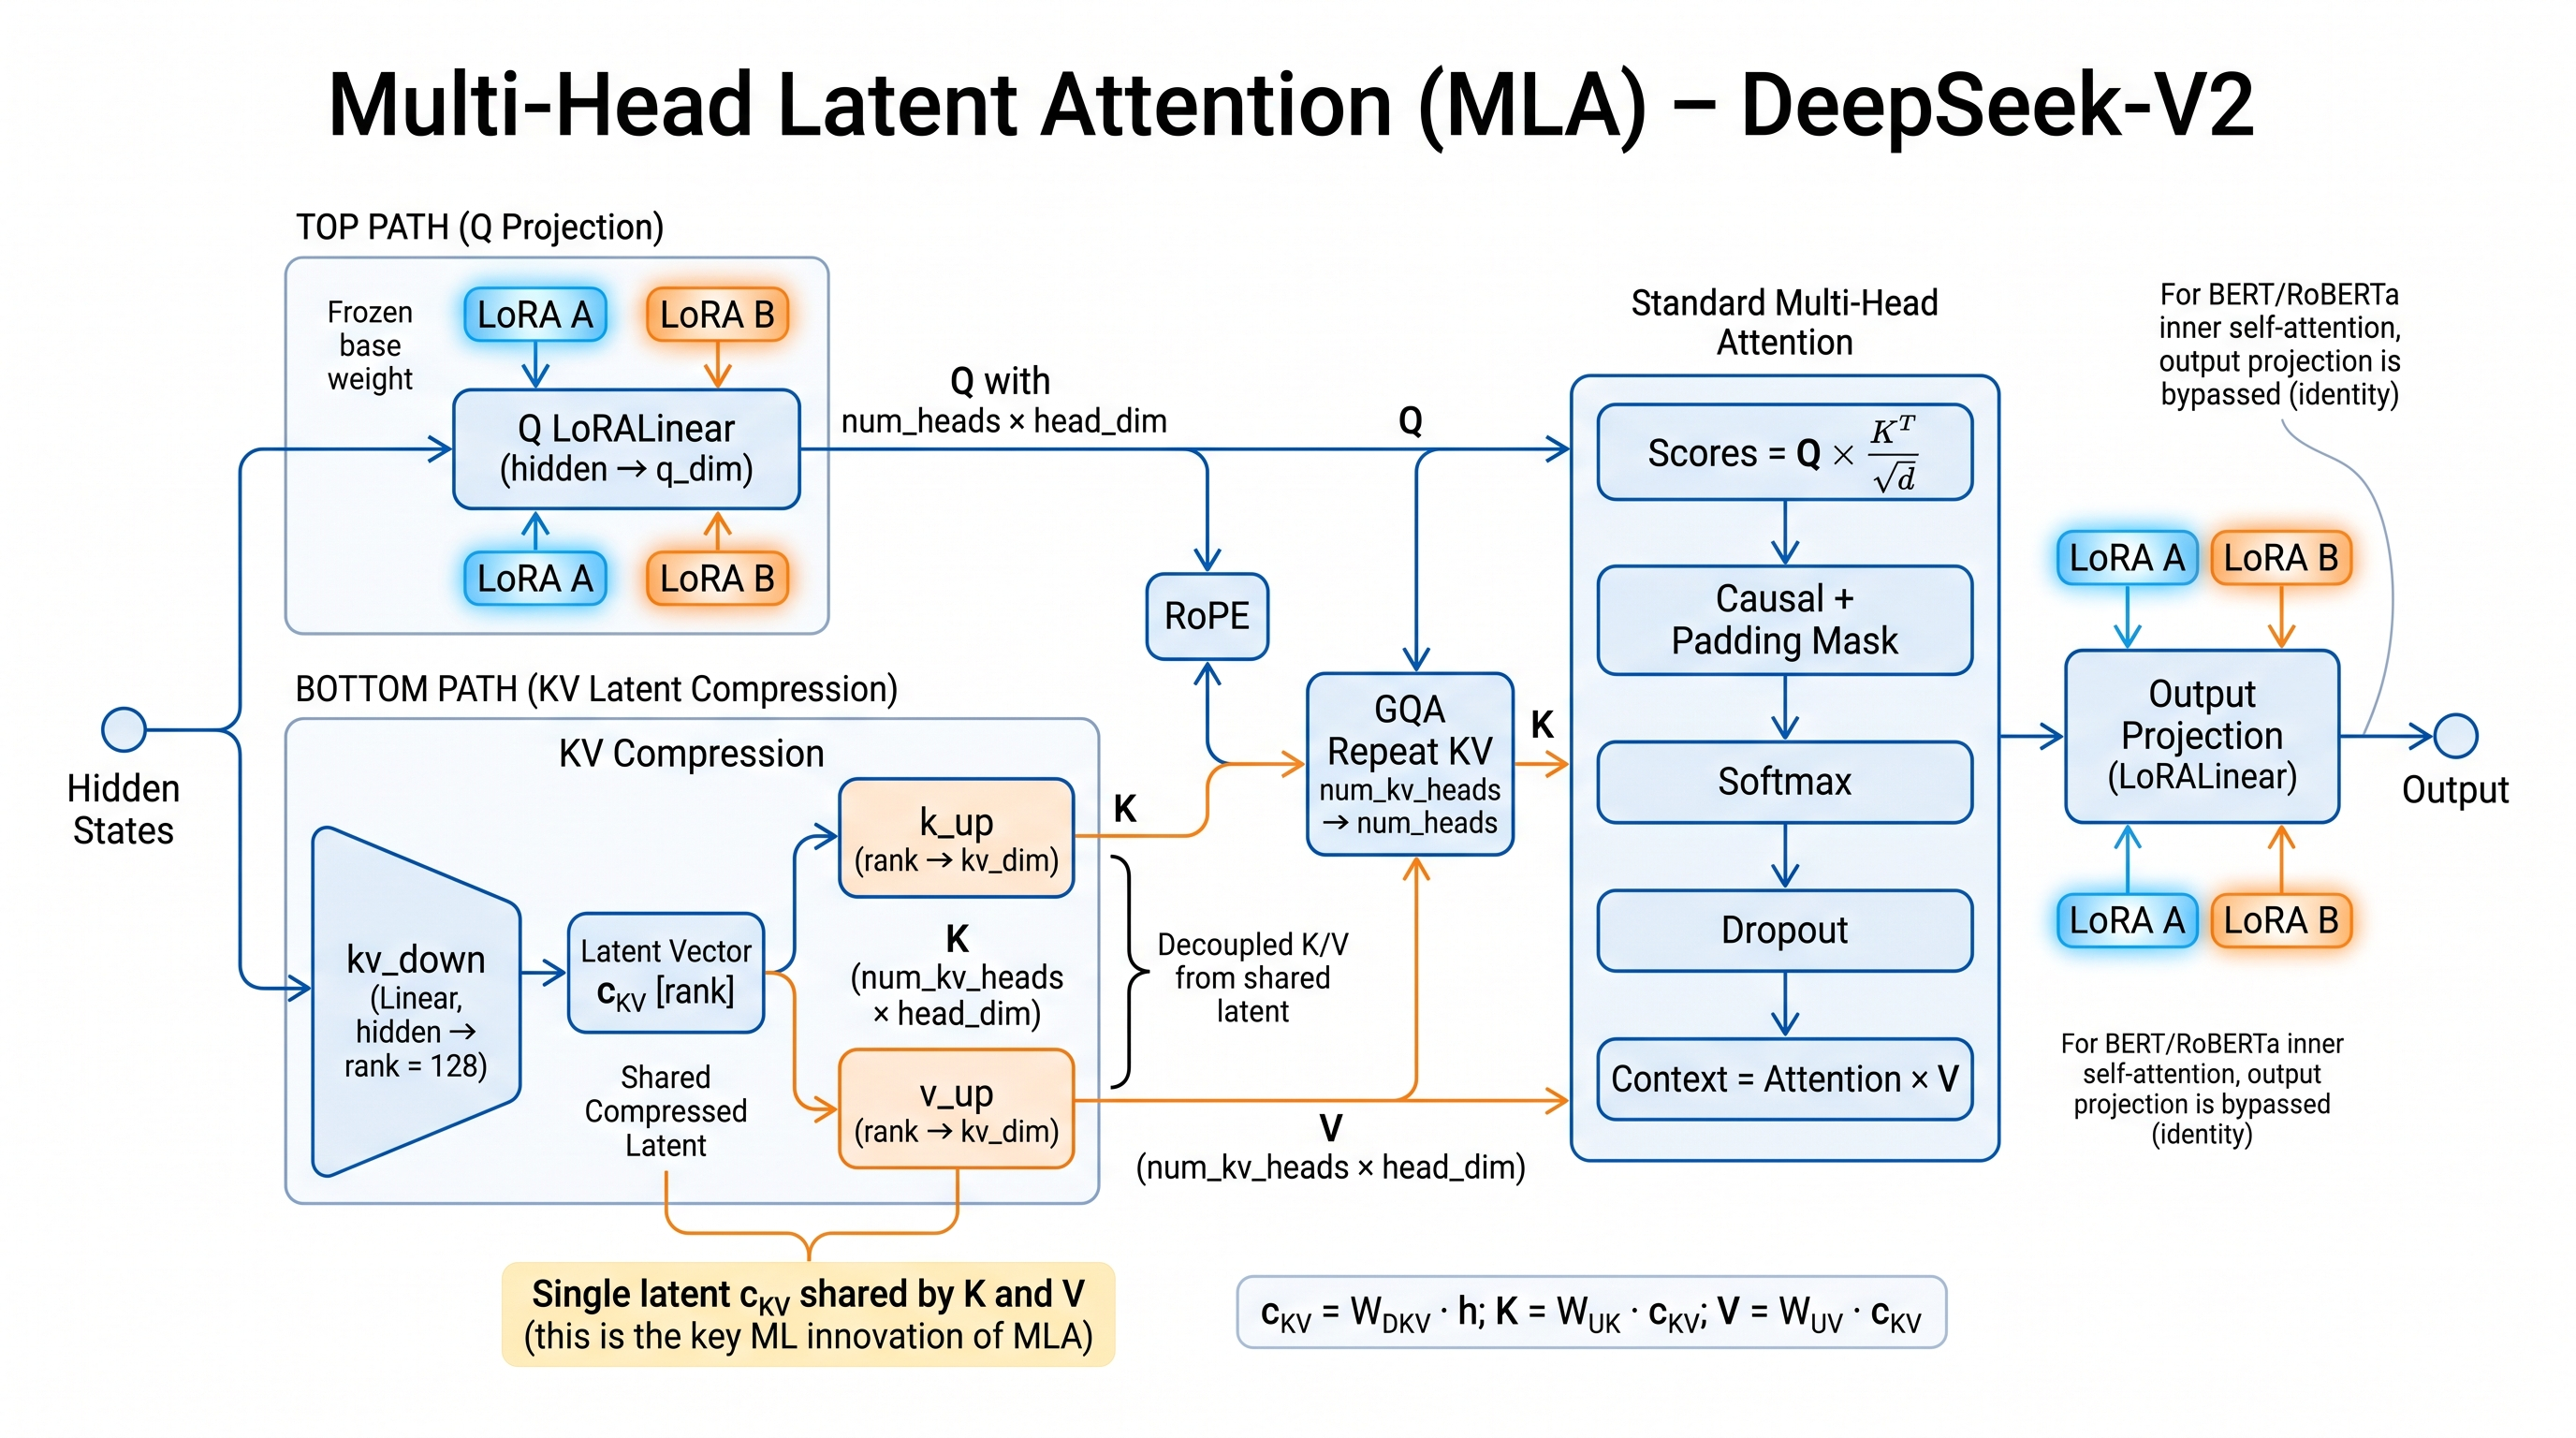
\includegraphics[width=\linewidth]{figures/architecture.jpeg}
\caption{High-level architectural diagram of mla\_attention.}
\label{fig:arch\_mla-attention}
\end{figure}

